\documentclass{standalone}
\usepackage{tikz}
\usepackage{verbatim}
\begin{document}
\pagestyle{empty}
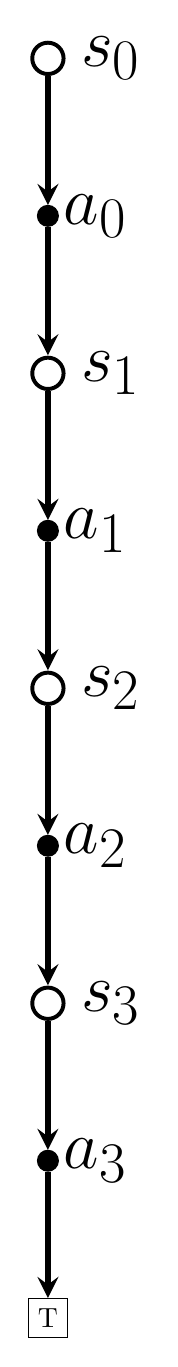
\begin{tikzpicture}

  % The graphic

  \foreach \xa in {3,2,1,0} {
      \node[draw,circle,scale=1.2, fill=white, line width=0.5mm] (s\xa) at (0,-4*\xa) {};
      \node at (0.8, -4*\xa) {\Huge $s_\xa$};
      \node[draw,circle,fill,scale=0.8] (a\xa) at (0, -4*\xa -2) {};
      \node at (0.6,  -4*\xa -2) {\Huge $a_{\xa}$};
      %\node[draw,circle,scale=0.6] (r\xa) at (\xa+.5,-2) {};
      \draw[-stealth, line width=0.8mm] (s\xa) -- (a\xa);
      %\draw[-stealth] (b\xa) -- (l\xa);
      %\draw[-stealth] (b\xa) -- (r\xa);
  }
  \node[minimum size=0.5cm, fill=white, draw] (s4) at (-0,-16) {T};
  \draw[-stealth, line width=0.8mm] (a0) -- (s1);
  \draw[-stealth, line width=0.8mm] (a1) -- (s2);
  \draw[-stealth, line width=0.8mm] (a2) -- (s3);
  \draw[-stealth, line width=0.8mm] (a3) -- (s4);
 
\end{tikzpicture}
\end{document}